% =============================================================================
% =============================================================================
% =============================================================================
\chapter{Field Line Resonance}
  \label{ch_flrs}

\todo{ULF, FLR, and Pc4 all mean basically the same thing in the context of the present work. How many acronyms do we really need? }

\todo{Other planets\cite{glassmeier_2004}? Seems exciting but maybe not relevant. }

The motion of a charged particle in a dipole field can be described in terms of three fundamental motions. First is cyclotron motion: a particle orbits around a magnetic field line in accordance with the Lorentz force. Second is bounce motion: while orbiting, the particle moves along the field line like a bead on a wire, back and forth between the northern and southern hemispheres\footnote{As a particle approaches Earth, it experiences an ever-stronger magnetic field. The particle's perpendicular kinetic energy increases in proportion with the magnetic field in order to conserve its first adiabatic invariant. When the perpendicular kinetic energy can no longer increase -- that is, when the parallel kinetic energy is zero -- the particle bounces back. (If the parallel kinetic energy is sufficiently large, the particle doesn't bounce; it precipitates into the atmosphere.)}. Third is drift motion: as particles orbit and bounce, they also move azimuthally around Earth per the gradient-curvature drift. 

Characteristic timescales for each of the above motions depend on particle energy. Electron cyclotron motion is on the order of \todo{$\cdots$} in the ionosphere, and closer to \todo{$\cdots$} in the tail; ions gyrate slower by three orders of magnitude due to their larger mass. \todo{Bounce... Drift... }

%\todo{Electron cyclotron frequency is on the order of $\sim \SI{1}{\MHz}$ in the ionosphere, and more like $\sim \SI{1}{\kHz}$ in the magnetosphere. Much faster than drift or bounce timescales. Ion cyclotron frequency... down by a factor of $\frac{\me}{\mp}$. }

%\todo{Bounce timescales are faster closer to Earth (where the field lines are short) and slower further out. Something like \SIrange{10}{100}{\second}. Bounce timescales depend only on velocity, right? }

%\todo{Drift timescales vary significantly based on particle energy. Dai\cite{dai_2013} showed a nice example of \SI{100}{\kilo\eV} ions drifting with a period of $\sim \SI{100}{\s}$. Bounce and drift timescales can overlap -- this turns out to be important. This doesn't depend on mass, right? Just kinetic energy. }

Wave-particle resonance arises when a particle's periodic motion matches with the frequency of a coincident electromagnetic wave\cite{elkington_1999,mann_2013,ozeke_2008,southwood_1976}. In the particle's rest frame, the wave then appears as a DC electric field. This allows a net movement of energy between the wave and the particle. The interaction is analogous to a surfer moving along with -- and being accelerated by -- a wave in the ocean. 

In the present work, the waves in question are field line resonances (FLRs). An FLR is a standing harmonic on a geomagnetic field line. It can also be envisioned as a superposition of traveling waves, reflecting back and forth between its northern and southern foot points at the conducting ionosphere. These waves travel at the \Alfven speed\footnote{The \Alfven speed is given by \va is given by $\va^2 \equiv \frac{B^2}{\mz \rho}$, where $B$ is the magnitude of the magnetic field, \mz is the magnetic constant, and $\rho$ is the mass density of the ambient plasma. It can vary by several orders of magnitude over the length of a magnetic field line. }. The fundamental equations of field line resonance were presented by Dungey in 1954\cite{dungey_1954}; since then, they have remained a topic of active study. 

So-called ultra low frequency waves  -- of which FLRs are a subset -- are categorized by morphology. Continuous (long-lived) pulsations are termed Pc, while irregular pulsations are called Pi. Within each are a number of frequency bands; see \cref{tab_iaga}\cite{jacobs_1964}. 

\begin{longtable}{ @{\extracolsep{\fill}} cccccccc @{\extracolsep{\fill}} }
  \caption[IAGA Magnetic Pulsation Frequency Bands]{IAGA Magnetic Pulsation Frequency Bands}
  \label{tab_iaga} \\
  \toprule
  & Pc1 & Pc2 & Pc3 & Pc4 & Pc5 & Pi1 & Pi2 \\
  \midrule
  \endfirsthead
  \bottomrule
  \endlastfoot
  Period (\si{\second}) & 0.2--5    & 5--10    & 10--45  & 45--150 & 150--600 & 1--40    & 40--150 \\
  Frequency (\si{\mHz}) & 200--5000 & 100--200 & 22--100 & 7--22   & 2--7     & 25--1000 & 7--25 \\
\end{longtable}

FLRs fall into the Pc3, Pc4, and Pc5 ranges. The present work focuses specifically on the Pc4 band: waves with periods of a minute or two. Frequencies in the Pc4 range typically coincide with \Alfven bounce times\footnote{The \Alfven frequency is the inverse of the \Alfven bounce time: $\frac{2 \pi}{\omega_A} \equiv \oint \frac{dz}{v_A}$. } near the plasmapause: $L\sim4$ to $L\sim6$\cite{anderson_1990,dai_2015,engebretson_1992,liu_2009}\footnote{Not coincidentally, these are the same $L$-shells where the Van Allen Probes spend most of their time; see \cref{ch_rbsp}. }. In fact, the large radial gradients in the \Alfven speed near the plasmapause act as an effective potential well, trapping FLRs\cite{dai_2009,klimushkin_2004,lee_1999,leonovich_2000,mager_2013,takahashi_2010}. 

In addition to being radially localized, FLRs in the Pc4 frequency band (also called Pc4 pulsations, or just Pc4s) are localized in MLT\footnote{MLT is Magnetic Local Time. Noon points toward the Sun and midnight away from it, with 06:00 and 18:00 at the respective dawn and dusk flanks. }. They have also been shown to occur preferrentially on the dayside\cite{anderson_1990,dai_2015,engebretson_1992,liu_2009,ukhorskiy_2005}. 

In the inner magnetosphere, the \Alfven frequency -- and thus the frequency of FLRs -- often coincides with integer or half-integer\footnote{See \cref{sec_harmonics}. } multiples of particle drift frequencies\cite{dai_2013}. The resulting wave-particle interactions can give rise to significant energization and radial diffusion of the particles\todo{Cite... everybody? }. In some cases, the waves also include an electric field parallel to the background magnetic field, contributing to the precipitation of energetic particles into the neutral atmosphere\cite{goertz_1979,goertz_1984,thompson_1996,wygant_2002}. 

The present chapter introduces the structural characteristics of FLRs, how those characteristics affect wave behavior, and several unresolved questions related to that behavior. 

%\todo{Parallel electric fields. In this regime, we're looking at inertial effects, not kinetic effects\cite{goertz_1979,thompson_1996}. Should produce non-monoenergetic precipitation, which are observed\cite{goertz_1984}. Consistent with MHD models\cite{chaston_2000,chaston_2002}. Inertial-scale structures observed with Polar\cite{wygant_2002}. }

%\todo{The plasmapause matters! Effective potential well, analogous to \Schrodinger's equation\cite{lee_1998,lee_1999,dai_2009}. Shown in theory\cite{klimushkin_1998,leonovich_2000,klimushkin_2004,mager_2013} and in observation\cite{takahashi_2009,takahashi_2010}.  }

%\todo{All sorts of FLR occur preferrentially (though not exclusively) on the dayside\cite{dai_2015,ukhorskiy_2005}. }

%\todo{Any waves with frequencies of $\SIrange{e-3}{1}{\Hz}$ are termed ULF waves -- ultra low frequency. ULF waves are furthermore categorized in terms of their morphological characteristics. Pc waves are continuous (exhibiting a fairly consistent waveform over a large number of wave periods) while Pi are irregular; the waves are further partitioned into frequency bands. See \cref{tab_iaga}. }

%\todo{These are Jacobs' original ranges... but are they really reflective of the jargon still used? It's weird that these ranges bottom out so far below 1000s. }

%\todo{While the IAGA characterizations are based on wave morphology, they do a decent job of deliniating between the different underlying physical processes as well. Pi2 pulsations (irregular waves with periods of a minute or two) tend to be excited on the nightside; they are associated with substorm onset (though the processes that give rise to Pi2s -- and their relation to substorm onset -- remains controversial). Pc1 and Pc2 pulsations tend to be EMIC (electromagnetic ion cyclotron) waves near the ion gyrofrequency, which are important for the precipitation of electrons (?). }

%Pi2: ``Clearly linked to substorm disturbances and other impulsive dynamics are the irregularly shaped waves in the 7--25-mHz band referred to as Pi2. Recent work on these waves suggests that their periodicity reflects the spectrum of global mode excitations of the plasmasphere but there is a competing proposal that the dominant frequencies are imposed by the modulated flows in the magnetotail.''\cite{kivelson_2006}

%\todo{The present work is specifically concerned with field line resonances near the plasmapause. These waves fall in the Pc4 range, with frequencies around \SI{10}{\mHz}\footnote{Notably, field line resonances can also fall within the Pc3 and Pc5 ranges. }. }

% Less than a decade later, Sigura presented observational evidence of the phenomenon: a wave seen simultaneously at the northern and southern foot points of a geomagnetic field line\cite{sigura_1961}. 

%\todo{There's no discussion of ULF frequency bands, or even use the term ``Pc4.'' That's probably a problem. Introduce \SIrange{7}{25}{\mHz}! }

% \todo{Pc4s are localized in L and in MLT\cite{anderson_1990,dai_2015,engebretson_1992,liu_2009}. Near the plasmapause. This is an important part of why the 2.5D model is a good fit! }

% -----------------------------------------------------------------------------
% -----------------------------------------------------------------------------
% -----------------------------------------------------------------------------
\section{Harmonic Structure}
  \label{sec_harmonics}

Wave structure along a geomagnetic field line is indicated by harmonic number. The first (or fundamental) harmonic has a wavelength twice as long as the field line. It exhibits an antinode in the perpendicular electric field at the equator, along with an antinode in the perpendicular magnetic field. The second harmonic is a single wavelength along the field line. Its perpendicular magnetic perturbation has an antinode at the equator, which its perpendicular electric field has a node. \cref{fig_harmonics} shows a qualitative sketch of each: a series of snapshots in time, in the rest frame of the wave. 

\begin{figure}[!htb]
    \centering
    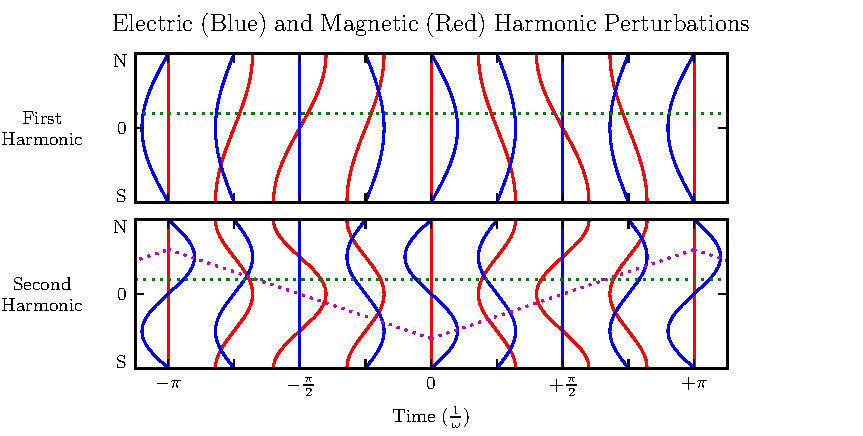
\includegraphics[width=\textwidth]{figures/harmonics.pdf}
    \caption[First and Second Harmonic Resonances]{
      The first (or fundamental) harmonic has an an antinode in its perpendicular electric field at the equator, along with a node in its perpendicular magnetic field perturbation. A single satellite can identify the first harmonic by the relative phase of the electric and magnetic field perturbations: an observer north of the equator (green) will see the electric field perturbation lead the magnetic field by \SI{90}{\degree}. The second harmonic is the opposite: it has an electric field node at the equator, and an observer north of the equator will see the electric field perturbation lag the magnetic field by \SI{90}{\degree}. The purple line sketches the path of a particle in drift-bounce resonance; in the particle's rest frame, the electric field is always to the right. 
    }
    \label{fig_harmonics}
\end{figure}

A first-harmonic FLR that is periodic or localized in the azimuthal direction is conducive to drift-resonant wave-particle interactions\cite{dai_2013,poulter_1983}. The particle is like a child on a swing: each time its orbit gets close to the wave (or parent), it gets a push, and always in the same direction. The wave fields spend half its time pointing the other direction, just as the parent must shift their weight backward to get ready for the next push, but at that point the particle (or child) is far away. 

Second-harmonic FLRs interact with particles through the drift-bounce resonance, which is slightly more complicated. As the particle drifts azimuthally, it also zig-zags north-south. The combination of those two periodic motions must align with the phase of the wave electric field. An example path is shown by the purple line in \cref{fig_harmonics}: the particle experiences a rightward electric field throughout the wave's oscillation. 

The drift-bounce resonance condition is written\cite{takahashi_2011}:
\begin{align}
  \omega - \azm \omega_D &= \omega_B
\end{align}

Where $\omega$ is the frequency of the wave, $\omega_D$ and $\omega_B$ are the particle's drift and bounce frequencies respectively, and \azm is the wave's azimuthal modenumber, as discussed in \cref{sec_azm}. 

In principle, the first and second harmonics can be distinguished by their frequencies, even from a single-point observation\cite{cummings_1969,green_1985}.  In practice, however, this is not a reliable approach\cite{takahashi_2013}. There are significant uncertainties surrounding the number density profile -- and thus the \Alfven speed profile -- along a geomagnetic field line. 

Harmonic structure can also be deduced by noting the phase offset between the wave magnetic field and its electric field (or the plasma velocity)\cite{takahashi_1992,dai_2015}. In \cref{fig_harmonics}, the green line indicates an observer just north of the magnetic equator. For the first harmonic, the observer sees the electric field waveform lead the magnetic field by a phase of \SI{90}{\degree}; for the second harmonic, the electric field waveform lags by \SI{90}{\degree}. (South of the equator, the signs are reversed.) Notably, this approach has only become viable with the advent of satellites carrying both electric and magnetic field instrumentation, such as THEMIS in 2007\cite{angelopoulos_2008} and the Van Allen Probes\footnote{The Van Allen Probes were previously called RBSP, for Radiation Belt Storm Probes. } in 2012\cite{stratton_2012}. 

Strictly speaking, the the phase offset of the electric and magnetic fields does not provide the harmonic number -- only its parity. It's reasonably safe to assume that an even mode is the second harmonic; the second harmonic is by far the most commonly observed\cite{hughes_1978,singer_1982,takahashi_1990}, due in part to the antisymmetric balloon instability\cite{southwood_1976,chen_1991,cheng_1994,chan_1994}. However, the distinction between the first and third harmonics is not always clear; this issue is discussed further in \cref{ch_rbsp}. Higher harmonics than that are not expected in the Pc4 frequency band. 

% Of 390 noncompressional events, Dai identified 19 to be clearly fundamental mode and 197 to be clearly second harmonic\cite{dai_2015}. 

\todo{Second-harmonic FLRs are unlikely to cause ground signatures\cite{takahashi_1992}. }

\todo{Dai found a nice event\cite{dai_2013} that was unambiguously determined to be a fundamental-mode Pc4 in drift-resonant interaction with \about\SI{e5}{\eV} ions. Consistent with \cite{thompson_2001}. Other observations of odd harmonics: \cite{yang_2010,eriksson_2005}. }

% -----------------------------------------------------------------------------
% -----------------------------------------------------------------------------
% -----------------------------------------------------------------------------
\section{Azimuthal Modenumber}
  \label{sec_azm}

The wavelength of an FLR in the azimuthal direction is indicated by its azimuthal wavelength. A wave with modenumber \azm has an azimuthal wavelength that spans $\frac{24}{\azm}$ hours in MLT. 

\begin{figure}[!htb]
    \centering
    
\includegraphics[width=\textwidth]{figures/placeholder.jpg}
    \caption[Large and Small Azimuthal Modenumbers]{
      \todo{$\cdots$}
    }
    \label{fig_azm}
\end{figure}

Waves with small azimuthal modenumbers ($0 < \azm < 10$) are typically driven by broadband energy sources at the magnetosphere's boundary, such as variations in the solar wind pressure\cite{zong_2007,zong_2009,hao_2014,degeling_2014,kessel_2008}, sporadic magnetic reconnection\cite{hughes_1994}, or Kelvin-Helmholtz waves on the magnetopause\cite{chen_1974,southwood_1974,liu_2011}. In the low-\azm regime, the shear and compressional \Alfven waves are coupled, which allows energy to move across field lines until the driving frequency lines up with the local \Alfven frequency\cite{lysak_1992}. Because of their broadband energy source, low-\azm FLRs often have a mishmash of frequencies present in their spectra\cite{dai_2015}.

When the azimuthal modenumber is large (or, equally, when the azimuthal wavelength is small), the shear and compressional \Alfven waves are decoupled\cite{cummings_1969,radoski_1974}\footnote{Equally, the strength of a wave's parallel component hint at its modenumber, a point which is revisited in \cref{ch_rbsp}. }. As a result, FLRs must be driven from within the magnetosphere. Proposed energy sources include phase space gradients near the plasmapause\cite{dai_2013}, particularly as the plasmasphere refills after a substorm\cite{engebretson_1992,liu_2013}. 

The ionosphere is known to attenuate waves with small spatial extent in the perpendicular direction\cite{hughes_1976,wright_1999,yeoman_2001}. As a result, FLRs may create no signature on the ground if their azimuthal modenumber is sufficiently large. For example, a recent paper by Takahashi shows a strong (\SI{2}{\nT} at $L\sim10$), clear resonance with \azm\about70 and no corresponding ground signature. 

% \todo{Waves with large \azm are screened by the ionosphere\cite{hughes_1976,wright_1999,yeoman_2001}. Observations of strong, clear waves in space have no corresponding ground signature when \azm is large\cite{takahashi_2013}. }

% \todo{Drift resonance with azimuthal wavenumber. In the analogy of a parent pushing a child on the swing, the child still gains energy even if the parent only shows up half the time. Or Are there a bunch of parents? The analogy starts to fall apart past there. }

%``To summarize, the general buffetting of the magnetosphere by variations in the solar wind dynamic pressure, or perhaps by sporadic magnetic reconnection, provides a broad band energy source to the magnetosphere. The magnetospheric cavity as a whole rings at its own eigenfrequencies, thus transporting energy at just those frequencies to field lines deep in the magnetosphere. Those field lines whose eigenfrequencies match one of the cavity eigenfrequencies couple to the cavity mode and resonate strongly, producing the classical field line resonance signature.\cite{hughes_1994}'' 

% Compressional driving doesn't preclude drift or drift-bounce resonance\cite{zong_2007,zong_2009}. 

% The strength of the compressional-poloidal coupling indicates \azm\cite{hughes_1994}. 

% Low-\azm waves tend to be more muddled... driven by broadband sources rather than resonance\cite{dai_2015}. 

% Small structures are also damped; resonances narrower than $\sim \SI{100}{km}$ aren't visible on the ground. See also Glassmeier and Stellmacher, 2000 (about small latitude). \Alfven waves with small latitudinal scale\cite{glassmeier_2000} are screened by the ionosphere. Attenuation factor from \cite{hughes_1976} and \cite{glassmeier_1984}. 

% -----------------------------------------------------------------------------
% -----------------------------------------------------------------------------
% -----------------------------------------------------------------------------
\section{Poloidal and Toroidal Polarizations}

Based on polarization, each FLR can be classified as either poloidal or toroidal. 

The poloidal mode is a field line displacement in the meridional plane, as shown in \cref{fig_poloidal}, with an accompanying electric field in the azimuthal direction. 

\begin{figure}[!htb]
    \centering
    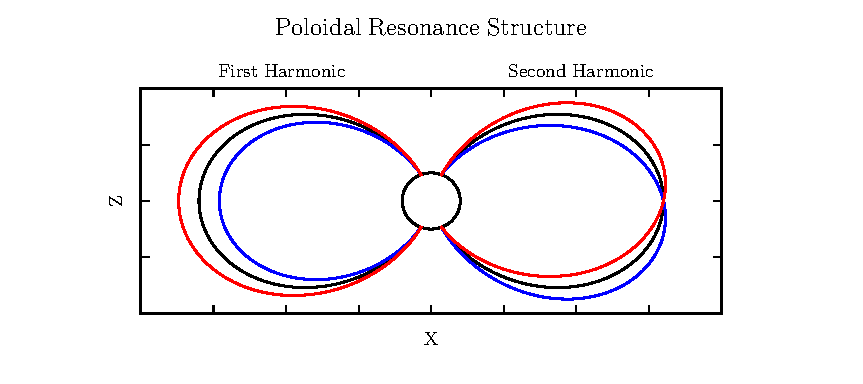
\includegraphics[width=\textwidth]{figures/poloidal.pdf}
    \caption[Poloidal Mode Structure]{
      The poloidal resonance is a magnetic field in the meridional plane. The displacement is radial near the equator, and can be accompanied by enhancement in the parallel magnetic field near the ionosphere. \todo{Lines are colored red and blue to contrast with the unperturbed black field line. }
    }
    \label{fig_poloidal}
\end{figure}

The toroidal mode's magnetic displacement is azimuthal, per \cref{fig_toroidal}; the associated electric field is in the meridional plane. 

\begin{figure}[!htb]
    \centering
    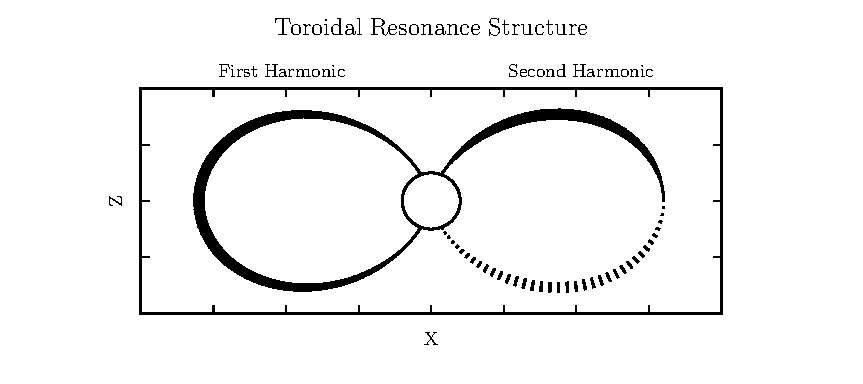
\includegraphics[width=\textwidth]{figures/toroidal.pdf}
    \caption[Toroidal Mode Structure]{
      A toroidally-polarized FLR has a magnetic perturbation in the azimuthal direction, as shown. Bold lines are taken to be above the page, and dotted lines below the page, with the displacement indicated by the line's width. 
    }
    \label{fig_toroidal}
\end{figure}

\todo{Toroidal modes are much more common\cite{anderson_1990}. }

\todo{The poloidal mode rotates to the toroidal mode in the presence of curved magnetic field lines\cite{radoski_1974} or a gradient in the \Alfven speed\cite{mann_1995}. The time is proportional to the azimuthal wavenumber\cite{mann_1995}. An analytical follow-up agreed with the numerical work\cite{mann_1997}. }

\todo{Fishbone instability? McGuire 1983, Chen 1984. Similar phenomenon, but for lab plasmas. }

\todo{Poloidal waves are more effective at creating ground signatures due to ducting by the ionosphere\cite{fujita_1988,greifinger_1968}. }

\todo{Poloidal and toroidal modes are coupled by the Hall conductivity\cite{kato_1956}. }

% -----------------------------------------------------------------------------
% -----------------------------------------------------------------------------
% -----------------------------------------------------------------------------
\section{Giant Pulsations}

\todo{First Pg observation\cite{birkeland_1901}. }

\todo{Giant pulsations are polarized in the meridional plane in space\cite{takahashi_1992}. However, due to the \about\SI{90}{\degree} rotation of long-period waves by the ionosphere\cite{nishida_1964_screening,hughes_1974}, they are primarily east-west polarized on the ground. }

\todo{Pgs are most common during solar minimum, perhaps because of decreased mass loading of heavy ions\cite{denton_2011}. }

\todo{The harmonic structure of giant pulsations was once controversial; at this point, there is general consensus (based on satellite data) that they are fundamental poloidal modes\cite{glassmeier_1999,hillebrand_1982,kokubun_1980,kokubun_1989,takahashi_1992,takahashi_2011}. }

\todo{Giant pulsations observed on the ground tend to have azimuthal modenumbers $10 \lesssim \azm \lesssim 40$\cite{glassmeier_1980,hillebrand_1982,poulter_1983,rostoker_1979,takahashi_1992}. }

\todo{Historically, the convention has been to identify giant pulsations by eye in ground magnetometer data, THEN look at satellite data? \cite{motoba_2015} }

\todo{Giant pulsations peak around \SI{66}{\degree} MLAT\cite{motoba_2015}, corresponding to L=6, but have been observed at $5 \lesssim L \lesssim 7$\cite{green_1985}. Most prevalent on the morningside, with some in the afternoon. }

\todo{Over the course of the twentieth century, a number of multi-year (sometimes multi-decade) surveys were published, tabulating nearly a thousand giant pulsation events (over 600 at Troms{\o}, Norway, alone!). On average, a ground magnetometer at \SI{66}{\degree} MLAT seems to observe 5 to 10 giant pulsations per year\cite{brekke_1987,harang_1941,rolf_1931,sucksdorff_1939}. The number depends on solar cycle as well as season. }

\todo{Giant pulsations preferrentially happen during quiet times, as the magnetosphere is recovering from previous activities\cite{motoba_2015,rostoker_1979}. Also notes that giant pulsations have no particular correlation with storm phase\cite{motoba_2015}. }


% Another past study: \cite{takahashi_1984_spectrum}. Satellite data is surveyed and classified by polarization, harmonic, wavenumber, etc, in order to determine the mechanisms for generating \Alfven waves. Old, but still pretty representative, according to Motoba\cite{motoba_2015}. 

% A long-period \Alfven wave passing through the ionosphere is rotated by about 90 degrees\cite{nishida_1964_screening,hughes_1974}. That would translate a poloidal resonance in space to an east-west ground signature. 

% \cite{motoba_2015} suggests that Pgs originate from the fundamental poloidal mode waves at all local times. 

% It seems to be the convention to find a Pg event on the ground, then look at satellite data. That's certainly what was done in \cite{motoba_2015}. 

% Per \cite{motoba_2015}, most Pg events happen around $L=7$, but some do happen near the plasmapause, as seen(?) by \cite{green_1985}. 

% ``The AL distribution shown in Figure 14c are consistent with the findings of \cite{rostoker_1979} that Pgs occur as the magnetosphere recovers from previous activities (substorms).''\cite{motoba_2015} Finds this to be reasonable because it's ``very likely'' that energetic ions injected into the inner magnetosphere from the magnetotail provide energy to Pgs. 

% Analysis of GOES data from 2008 to 2013 shows about 100 Pg events. They are concentrated on the morningside. No particular correlation with storm phase\cite{motoba_2015}. 

% Recall compressional poloidal Pc4s are mostly during storm time, and noncompressional are mostly specifically during late recovery\cite{dai_2015}. Only 19 fundamental poloidal mode examples were identified from the 390 noncompressional poloidal events. 

% -----------------------------------------------------------------------------
% -----------------------------------------------------------------------------
% -----------------------------------------------------------------------------
\section{Motivations for the Present Work}

Dai writes, in his 2015 paper\cite{dai_2015}, ``It is not clear why noncompressional [high-\azm] Pc4 poloidal waves, which are presumably driven by instability within the magnetosphere, preferrentially occur on the dayside.'' 

Motoba\cite{motoba_2015}, similarly, notes ``It is unclear whether other generation mechanisms of fundamental standing waves ... can explain the localization of Pgs in local time.''

The present work uses a numerical model to investigate the preferrential occurrence of field line resonances in the Pc4 range -- particularly first-harmonic poloidal modes, such as giant pulsations -- in MLT. 



Giant pulsations have variously been referred to as ``intriguing''\cite{green_1985}

``rare''\cite{brekke_1987}, even to the point of being ``a small subset of fundamental poloidal waves''\cite{takahashi_2013} -- note that it's well known that fundamental poloidal mode waves are already rare in comparison to second harmonic waves. 




\todo{What's going on with the MLT localization of Pc4 pulsations? Is there something spooky going on with the driving? Maybe the ionosphere just kills FLRs on the nightside! }

\todo{What's so special about Pgs? How rare are they, really, compared to fundamental poloidal modes in general? How does that line up with the occurrence rate of nice, sinusoidal waveforms in second-harmonic Pc4s? That is, is there something special about Pgs, or do they just live in a ``sweet spot'' with respect to constraints on observation and resonance? }

\todo{The goal here is to clarify and unify several constraints on the viability and observability of FLRs. }

%``Pgs maybe a manifestation of a small subset of fundamental poloidal waves excited in the magnetopause.'' \cite{takahashi_2013}

%``It is not clear why noncompressional [high-\azm] Pc4 poloidal waves, which are presumably driven by instability within the magnetosphere, preferrentially occur on the dayside.\cite{dai_2015}''

%``It is unclear whether other generation mechanisms of fundamental standing waves such as drift wave instability\cite{green_1979} can explain the localization of Pgs in local time (LT).''\cite{motoba_2015}








% Shear mode incident on the ionosphere, pederson current closes FAC, Hall current then generates a fast mode wave which may be detected in space or on the ground\cite{tamao_1965}. 

% Poloidal and toroidal ULF polarizations are treated differently by the ionosphere\cite{greifinger_1968} (more recently, \cite{fujita_1988}) due to ducting by the ionosphere. 

% In the example shown of a fundamental mode poloidal Pc4, and in the example of a higher harmonic Pc4, a mishmash of toroidal activity is present. \cite{dai_2015}, figure 8 and 9 respectively. 

% Observations of odd-mode poloidal waves... possible fundamental\cite{yang_2010,eriksson_2005}.

% \todo{Do the unambiguous Pc4 events in \cite{takahashi_2011} and \cite{dai_2013} also have a mishmash of toroidal activity? NO. }

% Poloidal Pc4s occur primarily during geomagnetically active times\cite{dai_2015}. This confirmed and refined older work\cite{engebretson_1987}. 

% Drift resonance happens when the bounce frequency of an \Alfven wave between the northern and southern ionospheres matches the bounce frequency of nearby particles. It allows the energization of ring current and radiation belt particles through drift and drift-bounce resonance\cite{elkington_1999,mann_2013,ozeke_2008,southwood_1976}. By multiple wave-particle interactions, poloidal ULF waves [FLRs] can lead to radial diffusion of radiation belt particles\cite{elkington_2003,ozeke_2012,tu_2012}.

%\begin{figure}[!htb]
%    \centering
%    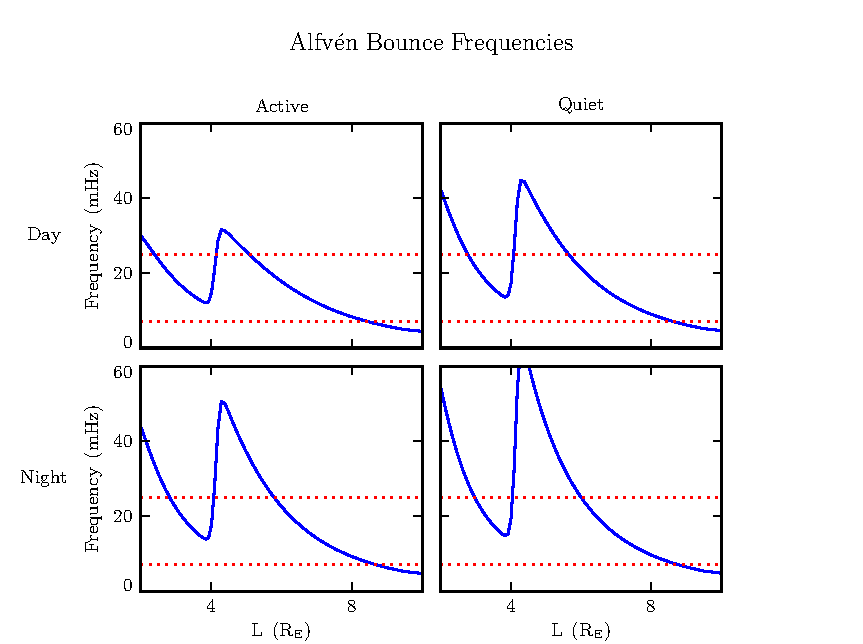
\includegraphics[width=\textwidth]{figures/fa.pdf}
%    \caption[\Alfven Bounce Frequency Profiles]{
%      \Alfven bounce frequency profiles, computed by integrating the the \Alfven speed back and forth over a field line. $f_A = \lrb{ \oint \frac{dz}{v_A} }^{-1}$. Dotted lines indicate the Pc4 frequency range, \SIrange{7}{25}{\mHz}. In each profile, the effect of the plasmapause is clearly visible, centered at $L=4$. Field lines just inside and just outside the plasmapause appear susceptible to resonance in the Pc4 band. \todo{Talk about how the size of the plasmasphere can be adjusted, and \SI{4}{\RE} is just a typical value. }
%    }
%    \label{fig_fa}
%\end{figure}

% ULF waves have been shown to correlate with pulsating aurora and with chorus\cite{jaynes_2015}. It's believed that (in the case presented) substorm injection drove Pc4-5 pulsations, which modulated chorus waves, which pitch-angle scattered electrons with energies on the order of \SI{10}{\kilo\eV}. 

% \todo{Theoretical consideration of decay vs propagation, by frequency. Lysak and Yoshikawa 2006. }

% Drift-wave instability\cite{hasegawa_1971,green_1979,green_1985} is also a possibility for exciting fundamental poloidal waves, though it requires cold plasma, so it could only happen in the plasmasphere. 

% AMPTE/CCE data has shown a correlation between poloidal Pc4 activity and intense ring current flux near the equator\cite{engebretson_1988}. 

% Toroidal mode is usually associated with external driving\cite{chen_1974,southwood_1974}. 

% A Hall-conducting ionosphere reflects ULF waves\cite{hughes_1974}. 

% Compressional poloidal Pc4 pulsations are much more common during storms, but not particularly sensitive to storm phase. Noncompressional ones occur primarily during recovery\cite{dai_2015,rostoker_1979,engebretson_1992,anderson_1994}. Note that Dai\cite{dai_2015} was pretty generous about what counted as a storm... anything that hits \SI{-30}{\nano\tesla}. So \cite{motoba_2015} may not have counted the same way when they found no particular correlation with storm phase. 





%
% From W J Hughes' Magnetospheric ULF Waves: A Tutorial With a Historical Perspective
%

% rolf 1920 for early observation of Pi2

% Patel 1965 made observations in space, and matched them to observations on the ground
% Cummings et al 1969 numerically integrated Dungey's equations to estimate eigenfrequencies
% soviets discovered that different pulsations have different sources in the 1970s; see troitskaya 1993 and greenstadt and russell 1993
% troitskaya 1969 showed that Pc3 can sometimes be explained by a sudden change in the size of the magnetosphere following an impulse. an example -- this must have also been seen earlier. because... 
% Bolshakova and Troitskaya 1968 showed that Pc3 observation depends on IMF N/S. Iff IMF is within about 50 degrees of the earth-sun linem Pc3 is observable on the ground. 
% Troitskaya et al 1971 showed Pc3 frequencies at L=3 depend on IMF magnitude
% Gul'elmi 1974 and Kovner et al gave theoretical justification for these observations. 
% Russell and Hoppe 1981 made observations upstream of the bow shock to unify some ideas. upstream waves are driven by ion cyclotron instability, which depends on IMF magnitude. 

% Gringauz et al 1970 found that solar wind number density affects Pc3 and Pc4 periods (oppositely). The Pc4 effect is a standing question. 

% Samson et al 1971 new observations with digital recording and arrays near the plasmapause! they showed MLT dependence of peak amplitude, and different regions of opposite circular polarization. 
% Dungey 1954 had suggested KH as a wave energy source, which explained the flipping circular polarization at noon. 
% Southwood 1974 went back to the equations and came up with a reason for resonance. waves hitting the bow shock propagate in as an evanescent fast mode. when it gets to a resonant field line, the fast mode couples to the shear mode. the energy tunnels. this only happens if dissipation is finite. 
% Chen and Hasegawa 1974 did too, independently
% Newton et al 1978 showed that joule dissipation at the ionosphere is dominant, and that the amount of dissipation determines the width of the resonance. 

% kivelson et al 1984 argued for cavity mode eigenfrequencies. Pc5. 
% kivelson and southwood 1985, 1986 did analytical work to defend it. 
% Lee and Lysak 1991 did numerical work in a dipole geometry. 

% Harrold and Samson 1992 The waves probably have to be reflected by the bow shock, not by the magnetopause, to line up with the observed eigenfrequencies. 1 to 3 mHz. 

% allan et al 1985 did early observation of ULF waves (Pc5 and Pc4) from waveform plots. 
% Waters et al 1991 ground-based observation of Pc3 and Pc4 before spacecraft existed at small L. 
% Menk et al 1993 also




